\documentclass[border=10pt]{standalone}
\usepackage[svgnames]{xcolor}
\usepackage{amsmath}
\usepackage{pgfplots}
\pgfplotsset{compat=newest}
\usepackage[sfdefault]{FiraSans}
\usepackage{FiraMono}
\renewcommand*\familydefault{\sfdefault}
\begin{document}
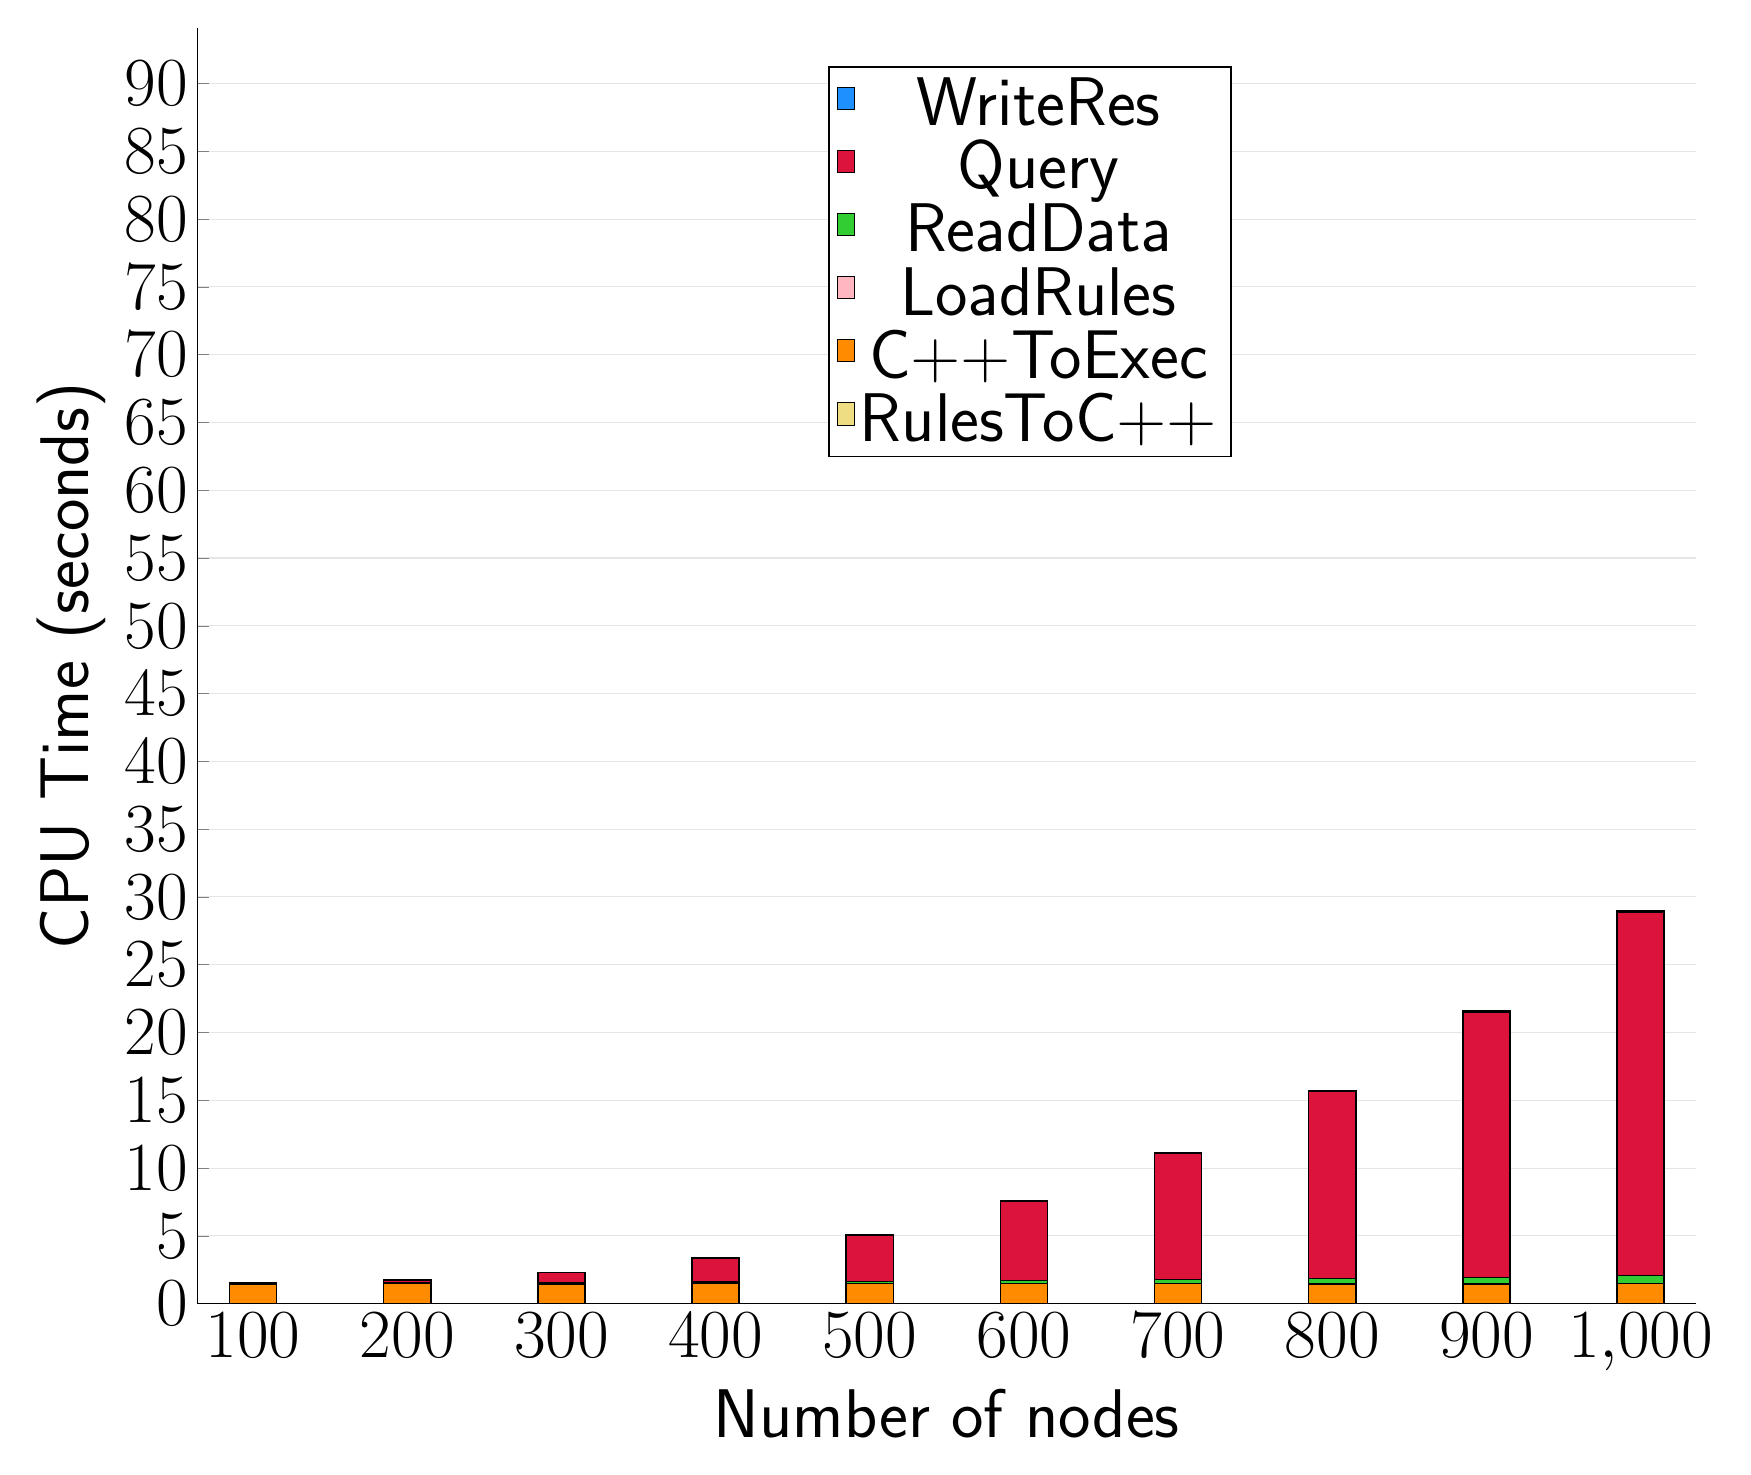
\begin{tikzpicture}
\begin{axis}[
   ybar stacked,
   width=1.7\textwidth,
   bar width=0.6cm,
   ymajorgrids, tick align=inside,
   major grid style={draw=gray!20},
   xtick=data,
   ymin=0, ymax=94.08204,
   axis x line*=bottom,
   axis y line*=left,
   enlarge x limits=0.04,
   legend style={
       at={(0.69, 0.97)},
       anchor=north east,
       legend columns=1,
       font=\Huge,
   },
   ylabel={CPU Time (seconds)},
   xlabel={Number of nodes},
   label style={font=\Huge},
   tick label style={font=\Huge},
]
\addlegendimage{fill=DodgerBlue, draw=black, line width=0.2pt}
\addlegendentry{WriteRes}
\addlegendimage{fill=Crimson, draw=black, line width=0.2pt}
\addlegendentry{Query}
\addlegendimage{fill=LimeGreen, draw=black, line width=0.2pt}
\addlegendentry{ReadData}
\addlegendimage{fill=LightPink, draw=black, line width=0.2pt}
\addlegendentry{LoadRules}
\addlegendimage{fill=DarkOrange, draw=black, line width=0.2pt}
\addlegendentry{C++ToExec}
\addlegendimage{fill=LightGoldenrod, draw=black, line width=0.2pt}
\addlegendentry{RulesToC++}
\addplot +[fill=LightGoldenrod, draw=black, line width=0.55pt] coordinates {
(100, 0.004000000000000001)
(200, 0.006000000000000001)
(300, 0.004000000000000001)
(400, 0.006000000000000001)
(500, 0.0020000000000000005)
(600, 0.008000000000000002)
(700, 0.004000000000000001)
(800, 0.004000000000000001)
(900, 0.006000000000000001)
(1000, 0.0020000000000000005)
};
\addplot +[fill=DarkOrange, draw=black, line width=0.55pt] coordinates {
(100, 1.462)
(200, 1.4679999999999997)
(300, 1.462)
(400, 1.472)
(500, 1.47)
(600, 1.466)
(700, 1.464)
(800, 1.4620000000000002)
(900, 1.4540000000000002)
(1000, 1.476)
};
\addplot +[fill=LightPink, draw=black, line width=0.55pt] coordinates {
(100, 0.0001538)
(200, 0.00016099999999999998)
(300, 0.00015759999999999998)
(400, 0.00016319999999999998)
(500, 0.0001574)
(600, 0.0001258)
(700, 0.0001676)
(800, 0.000154)
(900, 0.0)
(1000, 0.0001572)
};
\addplot +[fill=LimeGreen, draw=black, line width=0.55pt] coordinates {
(100, 0.0147896)
(200, 0.041839)
(300, 0.07426840000000001)
(400, 0.11435339999999998)
(500, 0.1649852)
(600, 0.22475879999999998)
(700, 0.3053518)
(800, 0.3890866)
(900, 0.4648958)
(1000, 0.5973258)
};
\addplot +[fill=Crimson, draw=black, line width=0.55pt] coordinates {
(100, 0.0431402)
(200, 0.2293734)
(300, 0.7472768000000001)
(400, 1.752296)
(500, 3.4048660000000006)
(600, 5.849704)
(700, 9.288908000000001)
(800, 13.80174)
(900, 19.59016)
(1000, 26.823040000000002)
};
\addplot +[fill=DodgerBlue, draw=black, line width=0.55pt] coordinates {
(100, 0.0014248)
(200, 0.0044564)
(300, 0.0099576)
(400, 0.0173284)
(500, 0.026957799999999997)
(600, 0.038592)
(700, 0.0522776)
(800, 0.06780800000000001)
(900, 0.0859326)
(1000, 0.10569139999999999)
};
\end{axis}
\end{tikzpicture}

\end{document}
